% !TEX program  = pdflatex
\documentclass{article}
\usepackage[ruled,vlined,linesnumbered]{algorithm2e}
\usepackage{algpseudocode}
\usepackage{amsmath}
\usepackage{amsthm}
\usepackage{graphicx}
\usepackage{subfigure}
\usepackage{float}
\usepackage{amsmath }
\usepackage{amsfonts }
\usepackage{pdfpages}
\usepackage{epsfig}
\usepackage{graphicx}
\usepackage{arydshln}
\usepackage{verbatim}
\usepackage{subfigure}
\usepackage{enumerate}
\usepackage{rotating}
\usepackage{threeparttable}
\usepackage{caption}
\usepackage{epsfig}
\usepackage{cite}
\usepackage{geometry}
\geometry{a4paper, top=2.54cm, bottom=2.54cm, left=3.18cm, right=3.18cm}
\theoremstyle{definition}
\newtheorem{prob}{Problem}
\newtheorem{ans}{Answer}
\usepackage[colorlinks,linkcolor=black]{hyperref}
\linespread{1.2}
\begin{document}
	\title{CS257 Linear and Convex Optimization Homework 7 Solution}
	\author{Kailing Wang 521030910356}
	\date{November 23.2022}
	\maketitle
	\begin{ans}
		~
		
		\begin{enumerate}[(a)]
			\item Differentiate the sum part of $\nabla f(\boldsymbol{w})$, which is $-\left[1-\sigma\left(y_i \boldsymbol{x}_i^T \boldsymbol{w}\right)\right] y_i \boldsymbol{x}_i$, we get
			
			$$
			\begin{aligned}
			y_i \boldsymbol{x}^T_i\sigma\prime\left(y_i \boldsymbol{x}_i^T \boldsymbol{w}\right)y_i\boldsymbol{x}_i\\
			=\sigma\prime\left(y_i \boldsymbol{x}_i^T \boldsymbol{w}\right)y_i^2\boldsymbol{x}^T_i\boldsymbol{x}_i
			\end{aligned}
			$$
			
			for $y_i\in \{-1,1\}$ is a label, $y_i^2=1$, so the second derivative of $f(x)$ is
			$$
			\nabla^2 f(\boldsymbol{w})=\sum_{i=1}^m \sigma^{\prime}\left(y_i \boldsymbol{x}_i^T \boldsymbol{w}\right) \boldsymbol{x}_i \boldsymbol{x}_i^T
			$$
			\item For case $w=(-1.5,1)^T$, the algorithm converges after 6 iterations. The results given is $w=(-1.87973941,2.601884520)$ and $\min f(w)$ is 3.3295135687527972. Figure \ref{p11} and \ref{p12} are the required plots. 
			
			\begin{figure}[h]
				\begin{minipage}[t]{0.5\linewidth}
					\centering
					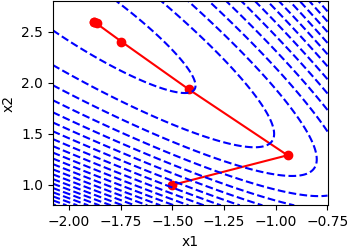
\includegraphics[width=0.9\linewidth]{../figures/1b/nt_traces0}
					\caption{Pure Newton: trajectory}
					\label{p11}
				\end{minipage}
				\begin{minipage}[t]{0.5\linewidth}
					\centering
					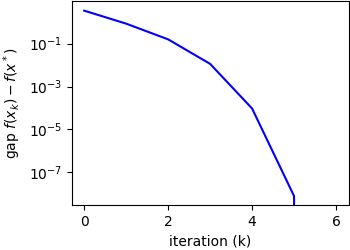
\includegraphics[width=0.9\linewidth]{../figures/1b/nt_gap0}
					\caption{Pure Newton: gap}
					\label{p12}
				\end{minipage}		
			\end{figure}
		
			For case $w=(1,1)^T$, the algorithm dose not converge because singular Hessian matrix is encountered. 
			\item Both cases converges. For case $w=(-1.5,1)^T$, the algorithm still converges after 6 iterations, and the results are completely the same with those of Pure Newton, for the back line search part is not used in this case. Figure \ref{p13}-\ref{p15} are required plots. No difference with Pure Newton's method is observed in this case. 
			
			\begin{figure}[h]
				\begin{minipage}[t]{0.33\linewidth}
					\centering
					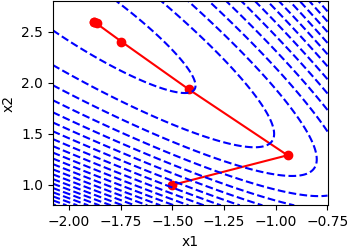
\includegraphics[width=1\linewidth]{../figures/1b/dnt_traces0}
					\caption{Damp: trajectory}
					\label{p13}
				\end{minipage}
				\begin{minipage}[t]{0.33\linewidth}
					\centering
					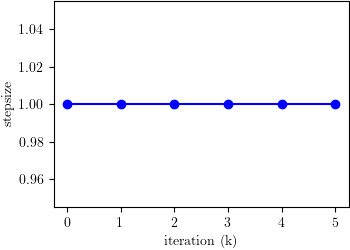
\includegraphics[width=1\linewidth]{../figures/1b/dnt_ss0}
					\caption{Damp: step size}
					\label{p14}
				\end{minipage}
				\begin{minipage}[t]{0.33\linewidth}
					\centering
					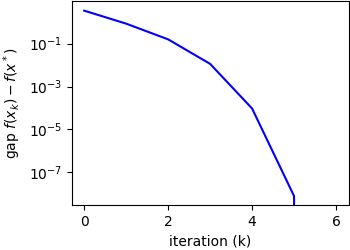
\includegraphics[width=1\linewidth]{../figures/1b/dnt_gap0}
					\caption{Damp: gap}
					\label{p15}
				\end{minipage}		
			\end{figure}
			
			For case $w=(1,1)^T$, the algorithm converges after 7 iterations. The results are $w=(-1.87973474,2.60187557)$, and $\min f(x)=3.3295135687768855$. Here significant difference occur because using Pure Newton we would come across singular matrix error. Figure \ref{p16}-\ref{p18} are required plots. 
			
			\begin{figure}[h]
				\begin{minipage}[t]{0.33\linewidth}
					\centering
					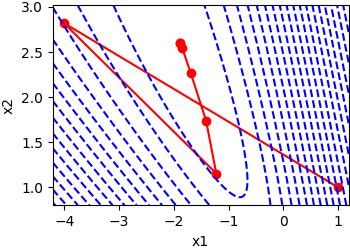
\includegraphics[width=1\linewidth]{../figures/1b/dnt_traces}
					\caption{Damp: trajectory}
					\label{p13}
				\end{minipage}
				\begin{minipage}[t]{0.33\linewidth}
					\centering
					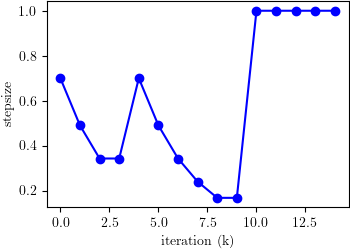
\includegraphics[width=1\linewidth]{../figures/1b/dnt_ss}
					\caption{Damp: step size}
					\label{p14}
				\end{minipage}
				\begin{minipage}[t]{0.33\linewidth}
					\centering
					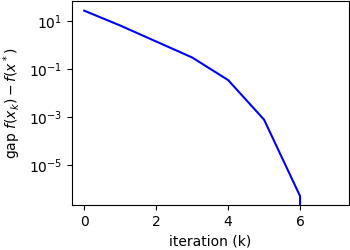
\includegraphics[width=1\linewidth]{../figures/1b/dnt_gap}
					\caption{Damp: gap}
					\label{p15}
				\end{minipage}		
			\end{figure}
		\end{enumerate}
	\end{ans}
	\begin{ans}
		~
		
		\begin{enumerate}[(a)]
			\item It seems that x is a scalar. Then $\nabla f(x)=6(x-a)^5$ and $\nabla^2 f(x)=30(x-a)^4$.
			\begin{algorithm}
				\caption{Newton's method}
				Initialization $x\gets x_0\in \mathbb{R}^n$\;
				\While{$||\nabla f(x)||>\delta$}
				{
					$\boldsymbol{x}\gets\boldsymbol{x}-[\nabla^2 f(\boldsymbol{x})]^{-1}\nabla f(\boldsymbol{x})$\;
					or $\boldsymbol{x}\gets\boldsymbol{x}-\frac{x-a}{5}$\;
				}
				\KwResult{$\boldsymbol{x}$}
			\end{algorithm}
			\item According to the algorithm above, we have 
			$$
			x_{new} = \frac{4x_{old}}{5}+\frac{a}{5}
			$$
			that is 
			$$
			x_{new} - a = \frac{4}{5}(x_{old} - a)
			$$ 
			now add abs on both side and we get 
			$$
			y_{k+1}=\frac{4}{5}y_k
			$$
			\item $\boldsymbol{x^*}=a$, according to the previous problem, 
			$$
			|x_{k+1}-a|=\frac{4}{5}|x_k-a|=(\frac{4}{5})^k|x_0-a|
			$$
			converges to 0 exponentially. 
		\end{enumerate}
	\end{ans}
	\begin{ans}
		~
		
		\begin{enumerate}[(a)]
			\item The solution is $w^*=(1.2, 0)$ with min value 4.9 after 31 iterations. The figure \ref{p31}, \ref{p32} are the required plots. 
			
			\begin{figure}[h]
				\begin{minipage}[t]{0.5\linewidth}
					\centering
					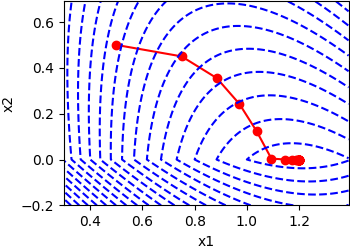
\includegraphics[width=0.9\linewidth]{../figures/4/ista_traces_lambda2}
					\caption{ISTA: trajectory}
					\label{p31}
				\end{minipage}
				\begin{minipage}[t]{0.5\linewidth}
					\centering
					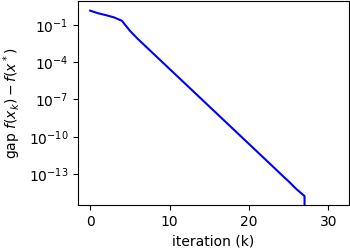
\includegraphics[width=0.9\linewidth]{../figures/4/ista_gap_lambda2}
					\caption{ISTA Newton: gap}
					\label{p32}
				\end{minipage}		
			\end{figure}
			
			\item Solution is $w^*=(1.69999998,-0.29999995)$ with min value 2.2500000000000004 after 927 iterations. Did not get zero in $w^*$. 
			\begin{figure}[h]
				\begin{minipage}[t]{0.5\linewidth}
					\centering
					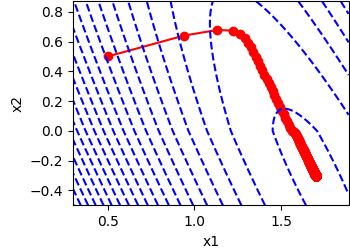
\includegraphics[width=0.9\linewidth]{../figures/4/ista_traces_lambda0.1}
					\caption{ISTA: trajectory}
					\label{p33}
				\end{minipage}
				\begin{minipage}[t]{0.5\linewidth}
					\centering
					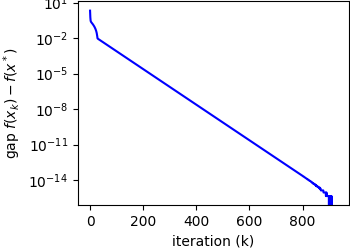
\includegraphics[width=0.9\linewidth]{../figures/4/ista_gap_lambda0.1}
					\caption{ISTA Newton: gap}
					\label{p34}
				\end{minipage}		
			\end{figure}
			
			\item Solution is $w^*=(1.11758702e-09,0.00000000e+00)$ with min value 8.5 after 28 iterations. This is almost 2 zeros. 
			
			\begin{figure}[h]
				\begin{minipage}[t]{0.5\linewidth}
					\centering
					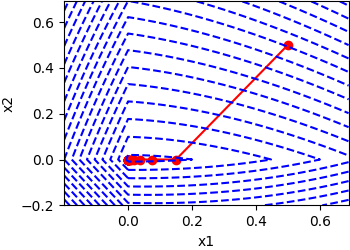
\includegraphics[width=0.9\linewidth]{../figures/4/ista_traces_lambda8}
					\caption{ISTA: trajectory}
					\label{p35}
				\end{minipage}
				\begin{minipage}[t]{0.5\linewidth}
					\centering
					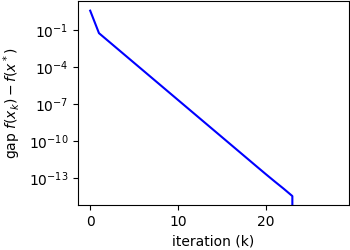
\includegraphics[width=0.9\linewidth]{../figures/4/ista_gap_lambda8}
					\caption{ISTA Newton: gap}
					\label{p36}
				\end{minipage}		
			\end{figure}
		
		\end{enumerate}
	\end{ans}
\end{document}